%!TEX program = pdflatex
% Full chain: pdflatex -> biber/bibtex -> pdflatex -> pdflatex
\documentclass[11pt,en]{elegantpaper}

\title{ECS659P/ECS7026P Project Report} 
\author{Bolun Xu 220234168}
% \institute{\href{https://github.com/ElegantLaTeX}{Elegant\LaTeX{} Program}}

% \version{0.11}
\date{Apr. 9, 2024}

% cmd for this doc
\usepackage{array}
\newcommand{\ccr}[1]{\makecell{{\color{#1}\rule{1cm}{1cm}}}}

\usepackage{graphicx} % 引入图片相关的包
\usepackage{subcaption}

% \addbibresource[location=local]{reference.bib} % reference file
\begin{document}

\maketitle

\section{Basic architecture}

The neural network model\footnote{All program code and historical models are publicly available on github! https://github.com/really-no-name/Neural-Networks-and-Deep-Learning-Project.git}applied in the remodelling project is a typical Convolutional Neural Network (CNN) used to classify the images in the CIFAR-10 dataset.The CIFAR-10 dataset contains $32\times32$ colour images in 10 categories. The network structure is defined in sequential layers (Sequential) and contains the following parts:

\subsection{Convolutional Layers}

\begin{itemize}
  \item The first layer is a convolutional layer with 64 filters (convolutional kernels), the kernel size is $3\times 3$ and a padding of 1 pixel is used to keep the image size constant.
  \item The second convolutional layer has 128 filters with the same kernel size and padding as above.
  \item The third convolutional layer has 256 filters with the same kernel size and padding.
\end{itemize}
  
These convolutional layers capture the features of the input image by applying filters. Each convolutional layer is followed by Batch Normalisation and ReLU activation functions to help the network learn non-linear features and accelerate training.
    
\subsection{Max Pooling Layers}

Each convolutional layer is followed by a Max Pooling Layer with a pooling region size of $2\times 2$ and a step size of 2. The Max Pooling Layers are used to reduce the size of the feature maps while retaining the most important features.

\subsection{Flatten Layer}

After all the convolutional layers, the feature map is flattened into a one-dimensional vector so that it can be processed by the fully connected layers.

\subsection{Fully Connected Layers}

\begin{itemize}
  \item The flattened layer is followed by a fully connected layer with 1024 neurons, followed by the ReLU activation function and the Dropout operation. The Dropout ratio is set to 0.6 to reduce overfitting and to increase the generalisation of the network by randomly discarding a portion of the neuron's outputs in each training iteration.
  \item Finally there is a fully connected layer with 10 output units corresponding to the 10 categories in the CIFAR-10 dataset. This layer will generate logits for classification, i.e., un-normalised prediction scores.
\end{itemize}

\section{Training techniques}

The entire network is trained using the CrossEntropyLoss function, which is a standard loss function for multi-class classification problems. The optimiser was chosen to be Adam, an adaptive learning rate optimisation algorithm widely used for training deep learning models. In addition, a learning rate decay strategy is used, which means that the learning rate is gradually reduced during the training process to help the model converge better.

\section{Training results}

\begin{figure}[htbp]
  \centering
\begin{subfigure}[b]{0.49\textwidth}
  \centering
  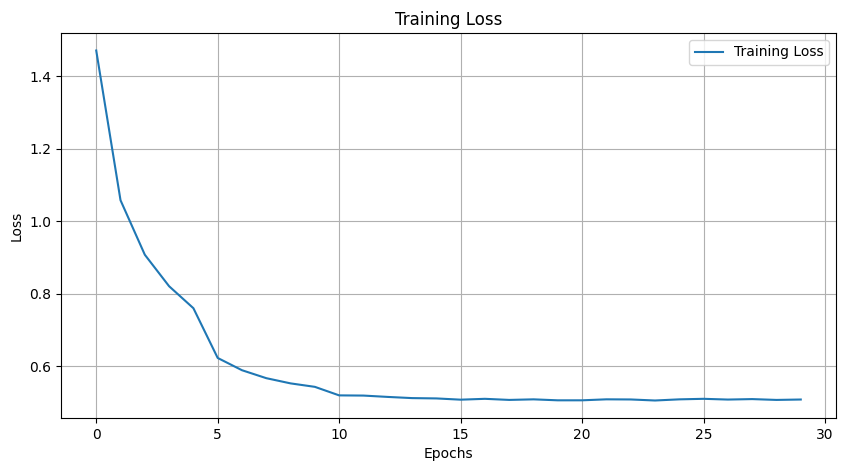
\includegraphics[width=\textwidth]{fig/Training_Loss.png}
  \caption{Training Loss}
  % \label{fig:sub1}
\end{subfigure}
\hfill
\begin{subfigure}[b]{0.49\textwidth}
  \centering
  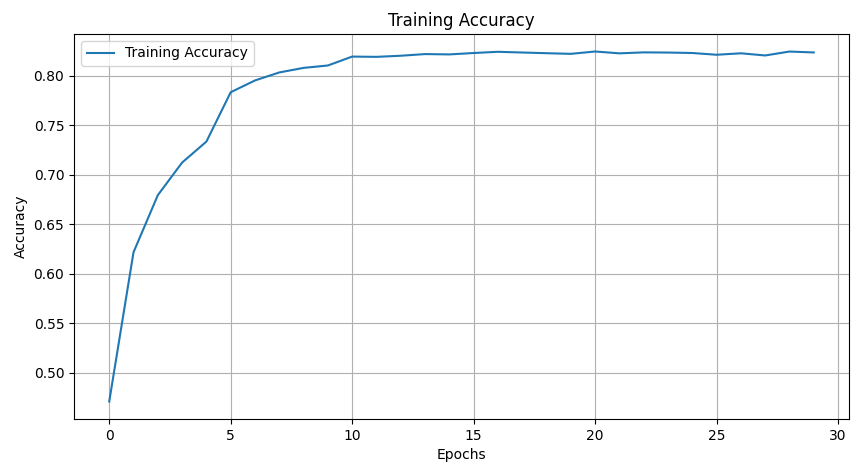
\includegraphics[width=\textwidth]{fig/Training_Accuracy.png}
  \caption{Training Accuracy}
  % \label{fig:sub2}
\end{subfigure}

\caption{Training Cycle}
% \label{fig:test}
\end{figure}


% \begin{figure}[htbp]
%   \centering % 使图片居中
%   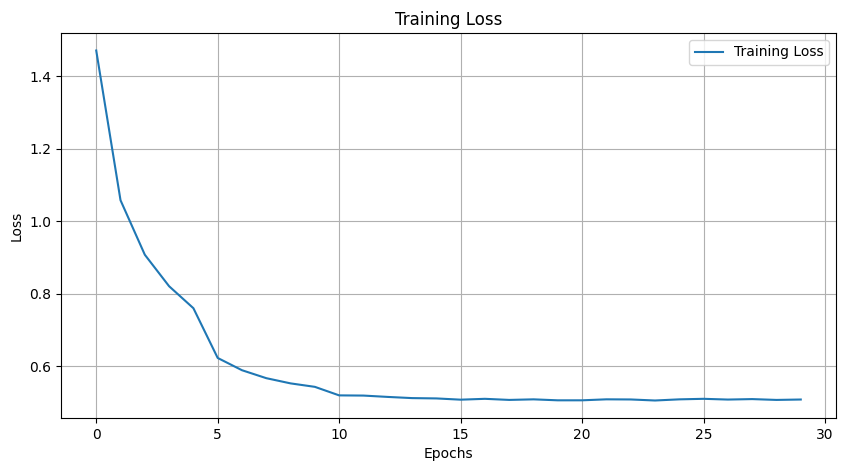
\includegraphics[width=0.7\textwidth]{fig/Training_Loss.png} % 图片文件的路径和名称
%   \caption{Training Loss}
%   % \label{fig:example}
%   \end{figure}

% \begin{figure}[htbp]
%   \centering % 使图片居中
%   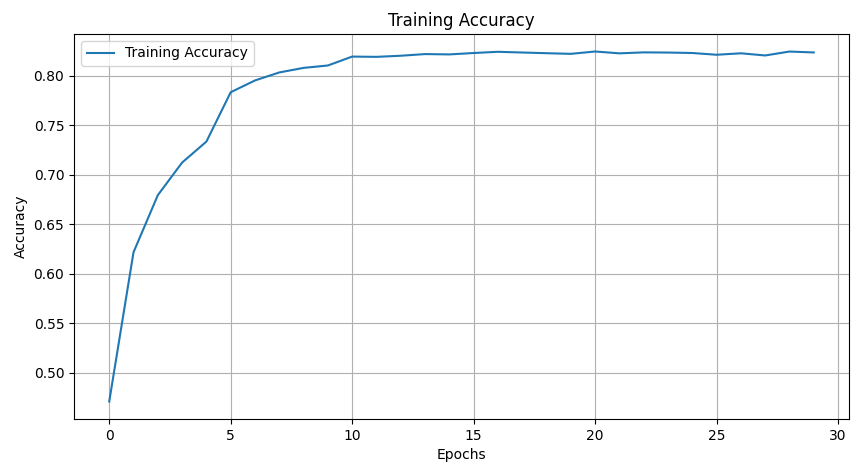
\includegraphics[width=0.7\textwidth]{fig/Training_Accuracy.png} % 图片文件的路径和名称
%   \caption{Training Accuracy}
%     % \label{fig:example}
% \end{figure}

\begin{figure}[htbp]
  \centering % 使图片居中
  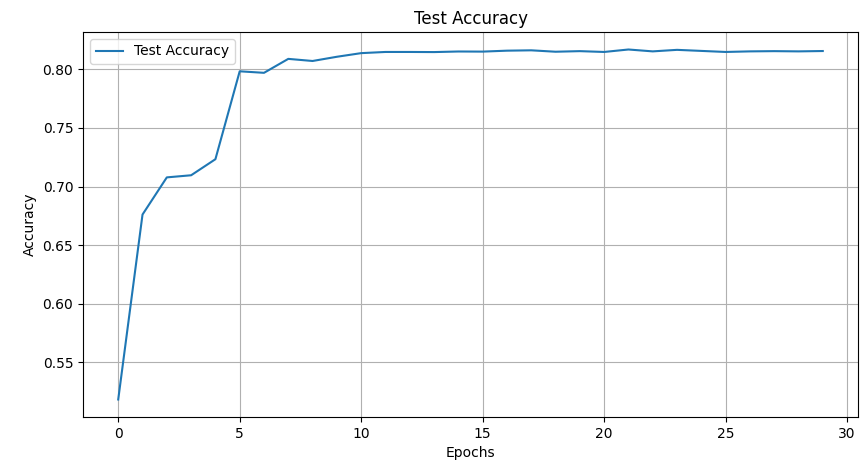
\includegraphics[width=0.7\textwidth]{fig/Test_Accuracy.png} % 图片文件的路径和名称
  \caption{Test Accuracy}
  % \label{fig:example}
  \end{figure}

Based on the results and output of the program running on the colab, the highest accuracy obtained by the neural network in the test dataset was \textbf{82\%}.

\section{Historical Record}

After the initial model construction, observations were recorded using TensorBoard. Based on the provided TensorBoard charts, the performance of the model during training can be analysed and model and parameter adjustments can be made:

\begin{itemize}
  \item \textbf{Add Data Augmentation}: In order to improve the generalisation of the model, more data augmentation techniques can be introduced such as rotation, translation, scaling, flipping, etc. This will help the model to be trained on more varied data, potentially improving the test accuracy.
  \item \textbf{Add Regularization}: If the model is overfitting, you can add regularisation terms (e.g. L1, L2 regularisation), or increase the Dropout ratio.
  \item \textbf{Learning Rate Decay}: If the training loss is starting to plateau, you can use a learning rate decay strategy, such as lowering the learning rate after every few epochs.
  \item \textbf{Modify Optimiser Parameters}: Try tweaking the parameters of the Adam optimiser, such as beta1, beta2 values or epsilon.
\end{itemize}

% \printbibliography[heading=bibintoc, title=\ebibname]

% \appendix
%\appendixpage
% \addappheadtotoc


\end{document}
